\documentclass{xjtureport}
\usepackage{graphicx}
\usepackage{float}
% =============================================
% Part 0 Edit the info
% =============================================

\major{大数据管理与应用}
\name{郅啸淇}
\title{最优化第三次作业}
\stuid{2184114639}
\college{管理学院}
\date{\zhtoday}
\lab{寝室}
\course{最优化理论与算法II}
\instructor{Xiangyu Chang}
\grades{??}
\expname{第三次作业题}
\exptype{完成作业}
\partner{Nobody}

\begin{document}
% =============================================
% Part 1 Header
% =============================================
\makecover

\makeheader

% =============================================
% Part 2 Main document
% =============================================

\section{HW1}
\subsection{Theorem1}
$D_{\phi }(x,y) + D_{\phi}(z,x) - D_{\phi}(z,y)$

$=\phi (x) - \phi (y) - \nabla \phi(y)^{T}(x-y) + \phi(z) - \phi(x) - \nabla\phi(x)^{T}(z-x) - \phi(z) + \phi(y) + \nabla\phi(y)^{T}(z-y)$

$=\nabla\phi(y)^{T}(z-y-x+y) - \nabla\phi(x)^{T}(z-x)$

$=(\nabla\phi(x) - \nabla\phi(y))^{T}(x-z)$

得证
\subsection{Theorem3}
由一般最优性条件$\langle \nabla f(x^{*}), y-x^{*} \rangle \geq 0$

则对于$D_{\phi}(x,y)$的最优值有$\langle \nabla D_{\phi}(x^{*},y) , (y-x^{*})\rangle \geq 0$

由条件有

$\pi ^{\phi}_{\omega}(y) = argmin_{x \in \omega} D_{\omega}(x,y)$

$\nabla D_{\phi}(x,y) = \nabla \phi(x) - \nabla \phi(y)$

代入$D_{\phi}$最优性条件即有

$(\nabla \phi(\pi_{\omega}^{\phi}(y)) - \nabla\phi(y))^{T}(\pi _{\omega}^{\phi}(y) -z) \leq 0 $

得证
\subsection{Theorem4}
由Theorem1有

$(\nabla \phi(\pi_{\omega}^{\phi}(y)) - \nabla\phi(y))^{T}(\pi _{\omega}^{\phi}(y) -z) = D_{\phi}(z,\pi _{\omega}^{\phi}(y))+ D_{\phi}(\pi_{\omega}^{\phi},y) - D_{\phi}(z,y) \leq 0$

故有$D_{\phi}(z,y) \geq D_{\phi}(z,\pi_{\omega}^{\phi}(y)) + D_{\phi}(\pi_{\omega}^{\phi}(y),y)$

得证
\section{HW2}

\subsection{Optimization of Quadratic Program}
\begin{equation}
    \begin{aligned} \label{P}
        & \min_{x} \frac{1}{2} \| \textbf{x}_0 - \textbf{x} \| ^2\\
        &\begin{array}[]{r@{\quad}r@{}l@{\quad}l}
        s.t.& A\textbf{x}_0 = \textbf{b}\\
        \end{array}
    \end{aligned}
\end{equation}

使用Lagrange乘数法,然后使用KKT条件求解$x^*$

$L(x,\lambda) = \frac{1}{2} \| \textbf{x}_0 - \textbf{x}\| + \lambda(A\textbf{x} - b)$

KKT条件

$\left\{\begin{matrix}
&\frac{\partial L}{\partial x} = -(\textbf{x}_0 - \textbf{x}) + A\lambda = 0\\
&\frac{\partial L}{\partial \lambda} = A\textbf{x} - b = 0\\
\end{matrix}\right.$

求解得

$\lambda = A(A^{T}A)^{-1} - (A^{T}A)^{-1}b$

$x^{*} = x_0 - A(A^{T}A)^{-1}(Ax_0-b)$

得证
\subsection{Projected Gradient Descent Algorithm}
上一题的二次规划最优解即向量对超平面的投影

即$\pi _c(x) = x - A(A^{T}A)^{-1}(Ax_0-b)$

那么优化问题

\begin{equation}
    \begin{aligned} \label{P}
        & \min_{x} f(x)\\
        &\begin{array}[]{r@{\quad}r@{}l@{\quad}l}
        s.t.& A\textbf{x}_0 = \textbf{b}\\
        \end{array}
    \end{aligned}
\end{equation}

的投影梯度下降迭代算法



\section{HW3}
\subsection{I}

$E_{D_{t}} \| g^{t} \| ^{2}=E \|\frac{1}{n_{b}} \sum_{i\in D_{t}} \nabla f_{i}(x^{t}) \| ^{2}$

$=\frac{1}{n_{b}^2}(\sum_{i\in D_{t}}^{n_{b}} E[\| \nabla f_{i}(x^t) \|^2] + \sum_{i\in D_{t},j\in D_{t},i \neq j}^{n_{b}} (E[\| \nabla f_{i}(x^t) \|^2] * E[\| \nabla f_{j}(x^t) \|^2]) )$

$=\frac{1}{n_{b}^2}(n_{b} \sigma ^{2} + n_{b}(n_{b} - 1) \|\nabla f(x^t)\| * \| \nabla f(x^t)\| )$

$=\frac{\sigma^2}{n_{b}} + \|\nabla f(x^t)\|^2$

得证

\subsection{II}
在A1条件下,有

$f(x^{t+1}) \leq f(x^t) + \langle \nabla f(x^t),x^{t+1} - x^{t} \rangle + \frac{\beta}{2} \|x^{t+1} - x^{t} \|^2$

$=f(x^t) -S_{t} \langle \nabla f(x^t),\nabla f_{i_{t}}(x^t) \rangle+ \frac{\beta S_{t}^{2}}{2}\| \nabla f_{i_{t}}(x^t)\| ^2 $

$=f(x^t) -S_{t} \langle \nabla f(x^t),\frac{1}{n_{b}}\sum_{i\in D_{t}} \nabla f_{i}(x^t) \rangle+ \frac{\beta S_{t}^{2}}{2}\| \frac{1}{n_{b}}\sum_{i\in D_{t}} \nabla f_{i}(x^t)\| ^2 $

对式子两边取期望,即得证。

\subsection{III}
在A1和A2的条件下

$E[f(x^{t+1})- f(x^t)] \leq \frac{\beta S_{t}^{2}}{2} E_{D_{t}}[\|g^t \|^2] - S_{t} \nabla f(x)^T E_{D_{t}}(g^t)$

$\leq \frac{\beta S_{t}^{2}}{2}(\frac{\sigma^2}{n_{b}} + \|\nabla f(x^t)\|^2) - S_{t} \|\nabla f(x^t) \|^2$

$=\frac{\beta S_{t}^{2}}{2n_{b}} \sigma ^2 - (s - \frac{\beta S_{t}^{2}}{2})\|\nabla f(x^t)\|^2$

得证
\subsection{IV}
在A1和A2的条件下

令$S_{t} \in (0,\frac{1}{\beta}]$

有引理

$f(x) - f^* \leq \frac{1}{2\alpha} \|\nabla f(x^t) \|^2$

则有

$E_{D_{t}}[f(x^{t+1}) - f(x^t)] = \frac{\beta S_{t}^{2}}{2n_{b}} \sigma^2 - (s - \frac{\beta S_{t}^{2}}{2})\|\nabla f(x^t) \|$

$\leq \frac{\beta S_{t}^{2}}{2n_{b}} \sigma^2 - \alpha S_{t}(f(x^t) - f^*)$

$\Rightarrow E_{D_{t}}[f(x^{t+1}) - f^* + f^* - f(x^t)] \leq \frac{\beta S_{t}^{2}}{2n_{b}} \sigma^2 - \alpha S_{t}(f(x^t) - f^*)$

$\Rightarrow E_{D_{t}}[f(x^{t+1}) - f^*] \leq \frac{\beta S_{t}^{2}}{2n_{b}} \sigma^2 - (1-\alpha) S_{t}(f(x^t) - f^*)$

$\Rightarrow E_{D_{t}}[f(x^{t+1}) - f^*] - \frac{\beta S_{t}}{2n_{b}\alpha (2-\beta S_{t})} \sigma^2 \leq \frac{\beta S_{t}^{2}}{2n_{b}} \sigma^2 - \frac{\beta S_{t}}{2n_{b}\alpha (2-\beta S_{t})} \sigma^2 + (1-\alpha) S_{t}(f(x^t) - f^*)$

$\leq (1- \alpha S_{t}(2 - \beta S_{t}))(f(x^t) - f^* - \frac{\beta S_{t}}{2n_{b}\alpha (2-\beta S_{t})} \sigma^2)$

对两边取期望即得证
\section{HW4}
逻辑回归对应的优化问题可以写成

$\mathop{\min}_{x\in \textbf{R}} = \frac{1}{N} \sum_{i=1}{N} f_{i}(x) = \frac{1}{N} \sum_{i =1}{N} ln(1+exp(-b_{i}*a_{i}^{T}x)) + \lambda \| x\|_{2}^{2}$
\lstinputlisting[language=Python]{code/SGD12+SVRG.py}
\begin{figure}[H]
    \centering
    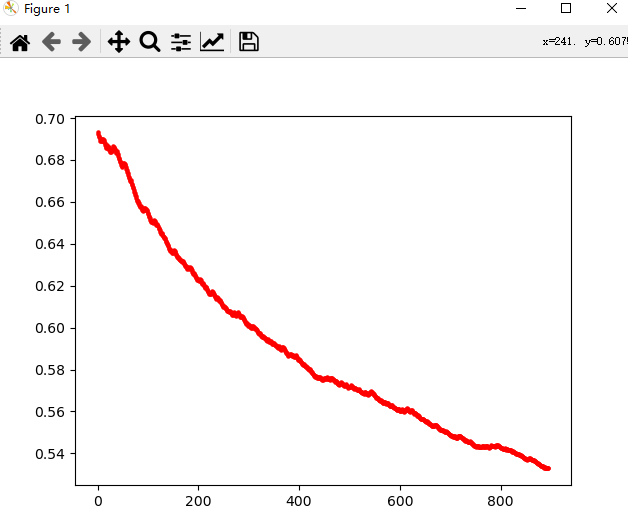
\includegraphics[scale = 0.4]{Fixed Step SDG.png}
    \caption{Result of Fixed Step SDG}
    \end{figure}
\begin{figure}[H]
    \centering
    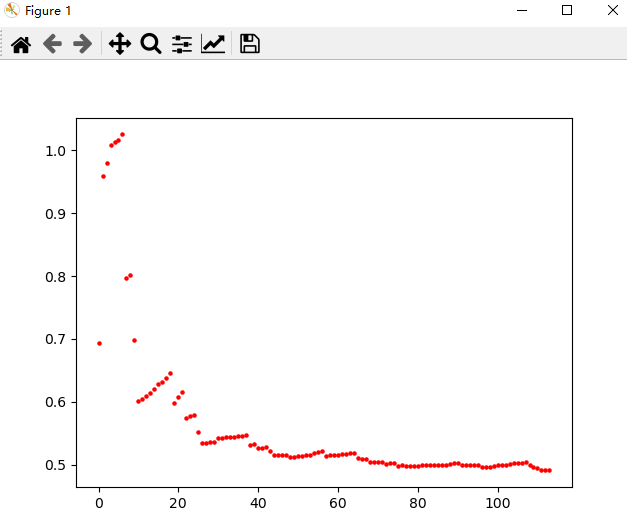
\includegraphics[scale = 0.4]{Descent Step SDG.png}
    \caption{Result of Descent Step SDG}
    \end{figure}
\begin{figure}[H]
    \centering
    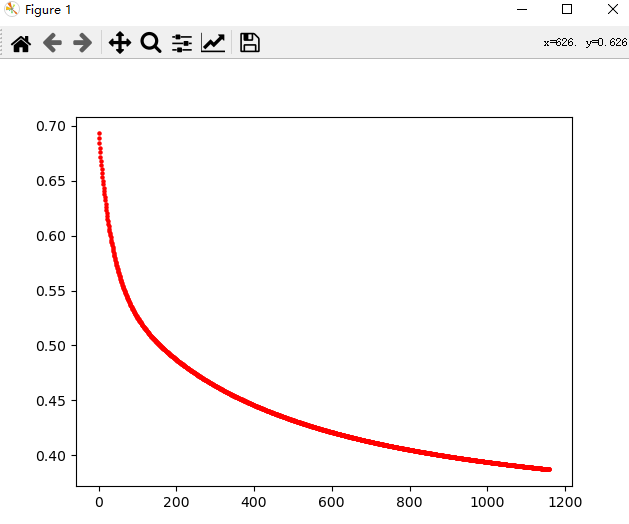
\includegraphics[scale = 0.4]{SVRG.png}
    \caption{Result of SVRG}
    \end{figure}
\end{document}
